%\chapter{Marco te\'orico}

\section{Descripci\'on de la Empresa}

Grupo Electrobodegas pertenece a un grupo de empresas hermanas, que se dedican a comercializar productos eléctricos de baja, mediana y alta tension. Cuenta con un gran numero de clientes entre ellos personas, empresas, alcaldías, ONG’s, Gobierno Central, ademas compite en licitaciones para adjudicarse proyectos estatales de presupuesto mediano y grande.

\begin{center}
  Sitio web de Electro Bodegas: \url{http://www.electrobodegas.com/}

  \begin{figure}[h!]
    \centering
    
\includegraphics{electrobodegas}
    \caption{Logo de Electro Bodegas}
  \end{figure}
\end{center}

\\
\textbf{Ubicaci\'on:}

\begin{figure}
  \centering
  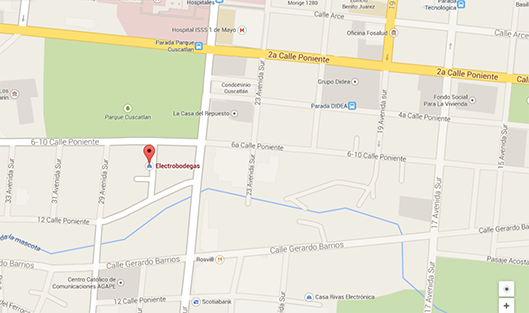
\includegraphics{electromap}
  \caption{Mapa de ubicación de Electro Bodegas (Vista satélite Google maps)}
\end{figure}

La empresa se encuentra en una ubicación accesible desde varios puntos de la capital, en la 27 av. Sur y $6\degree$ $10\degree$ calle poniente, al sur del parque Cuscatlan.

\textbf{Empresas hermanas:}

\begin{TAB}(r, 5pt, 1cm)[30pt]{cc}{cc}
  \vtop{
    \hbox{\strut 
\includegraphics[scale=0.3]{surtielectric}}
    \hbox{\strut \textbf{Surtielectric}}
    \hbox{\strut Ubicación: Av. España y}
    \hbox{Alameda Juan Pablo II los Próceres.}}
  &
  \vtop{
    \hbox{\strut 
\includegraphics[scale=0.3]{csh-logo}}
    \hbox{\strut \textbf{Csh Ingeniería}}
    \hbox{\strut Ubicación: Av. España y Alameda}
    \hbox{Juan Pablo II los Próceres.}}
  \\
  \vtop{
    \hbox{\strut 
\includegraphics[scale=0.3]{tecnelec}}
    \hbox{\strut \textbf{Tecnelec}}
    \hbox{\strut Ubicaci\'on: San Miguel.}}
  &
  \vtop{
    \hbox{\strut 
\includegraphics[scale=0.3]{pelsa-logo}}
    \hbox{\strut \textbf{Pelsa Panama}}}
  \\
\end{TAB}

%%% Local Variables:
%%% mode: latex
%%% TeX-master: "../virtualizacion"
%%% End:
